\section{Gestione arco}
Per quanto riguarda la gestione degli archi, l'utente ha la possibilità di:
\begin{itemize}
	\item aggiungere un \mglo{Arco}{arco};
	\item visualizzare i dettagli relativi a un certo arco presente;
	\item modificare un arco presente;
	\item eliminare un arco presente;
\end{itemize}

\subsection{Aggiunta di un arco}
Per aggiungere un arco si deve:
\begin{itemize}
	\item cliccare sul pulsante "+" in basso a destra della mappa;
	\item selezionare la voce "Aggiungi arco";
	\item selezionare il nodo di inizio e il \mglo{Nodo}{nodo} di fine sulla mappa;
	\item cliccare sul pulsante "Salva", che verrà abilitato solo nel momento in cui tutte le operazioni sopra descritte sono state eseguite in maniera corretta.
\end{itemize}

\begin{figure}[H]
\centering
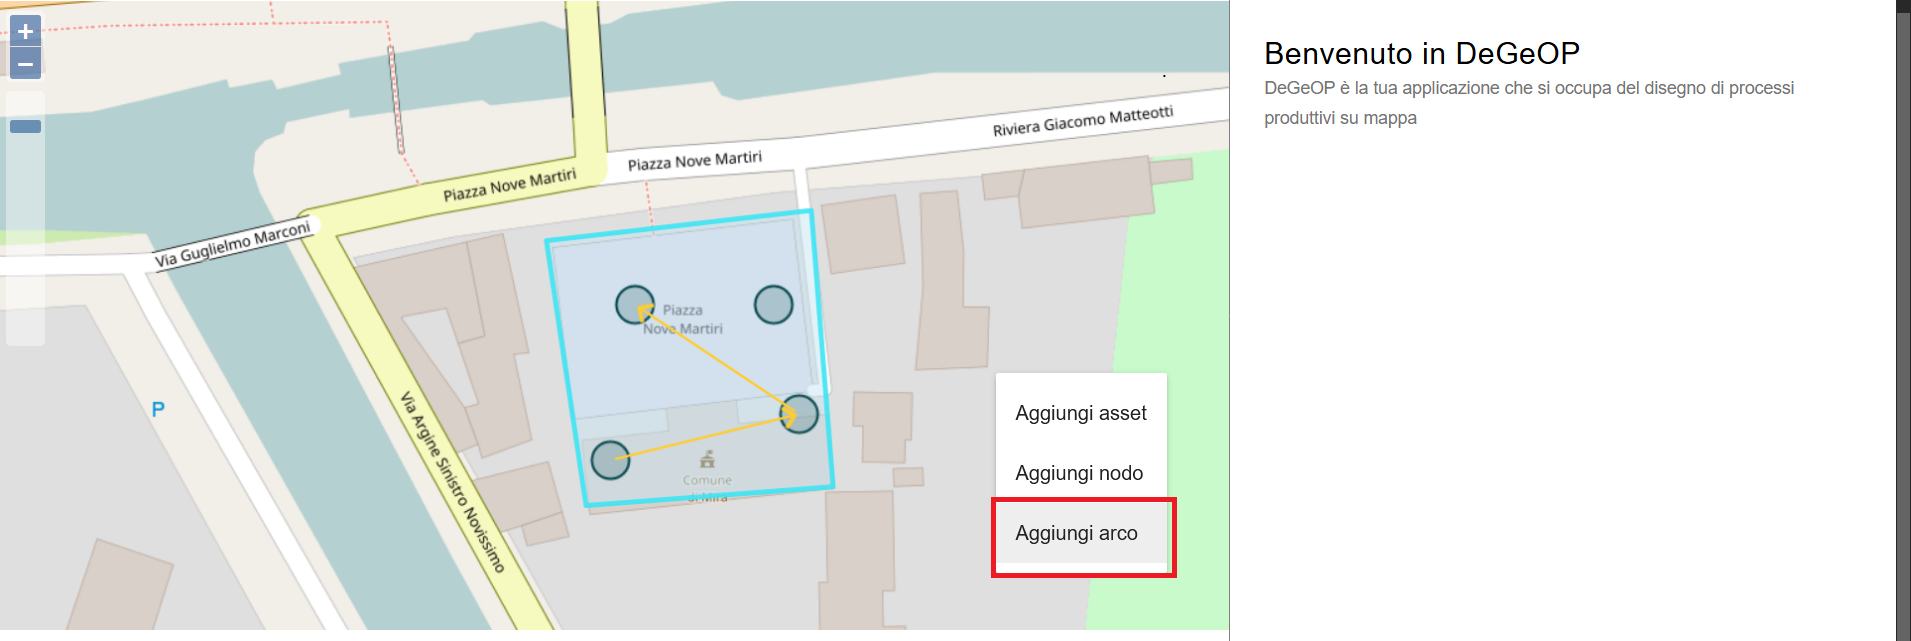
\includegraphics[width=\textwidth]{img/menu_aperto_arco_hover.png}
\caption{Menu di aggiunta}
\end{figure}

\begin{figure}[H]
\centering
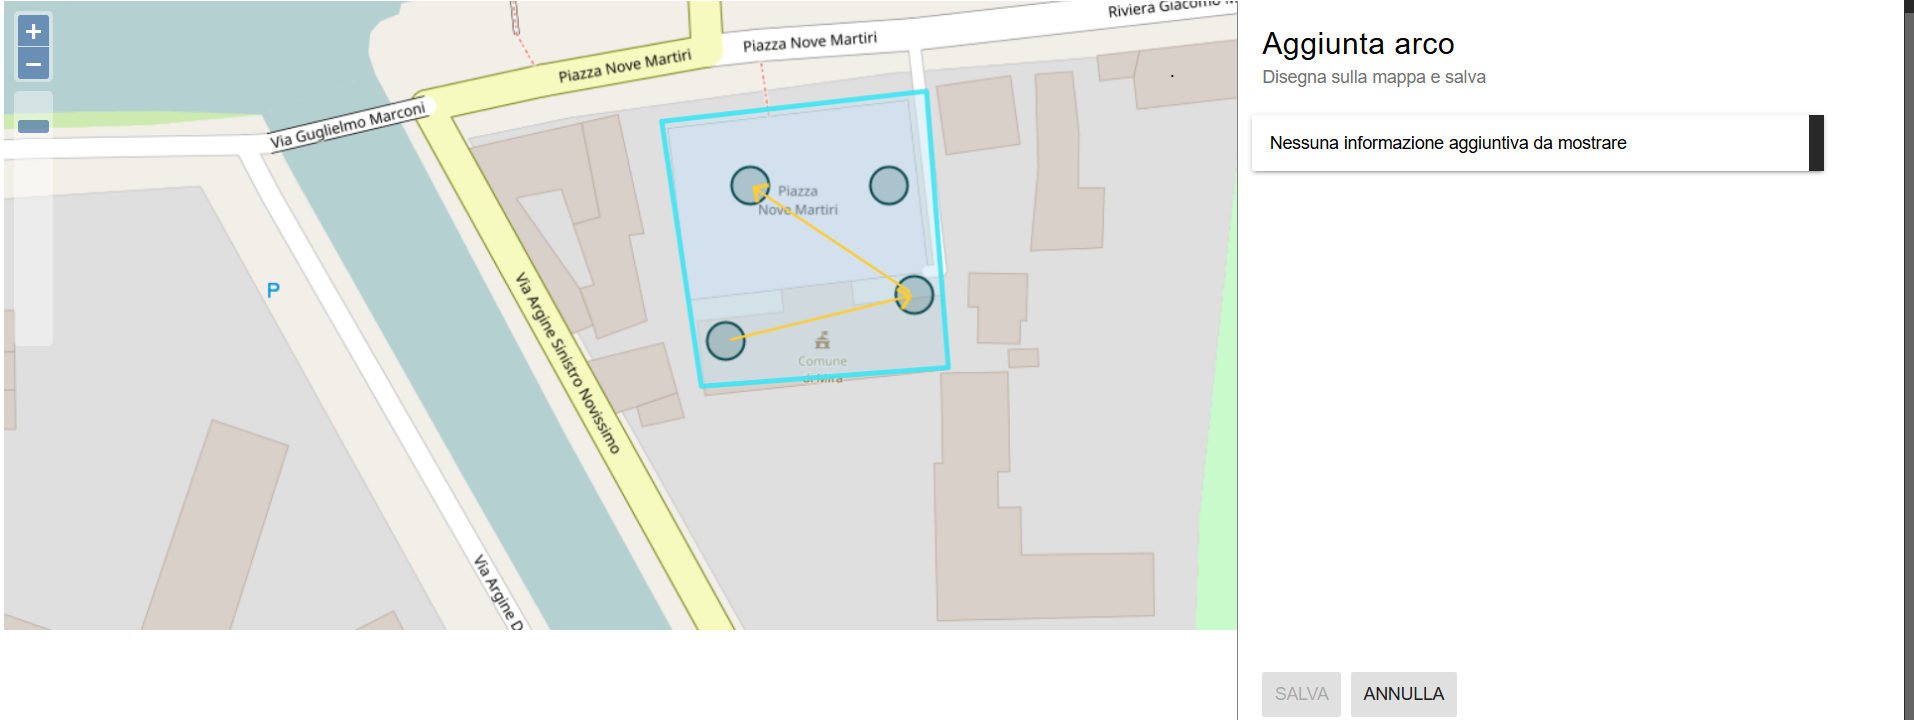
\includegraphics[width=\textwidth]{img/aggiunta_arco.png}
\caption{Aggiunta di un arco}
\end{figure}

\subsection{Visualizzazione dei dettagli di un arco}
Per visualizzare i dettagli di un arco si deve:
\begin{itemize}
	\item selezionare l'arco che si intende modificare cliccando direttamente su quell'arco dalla mappa.
\end{itemize}

\begin{figure}[H]
\centering
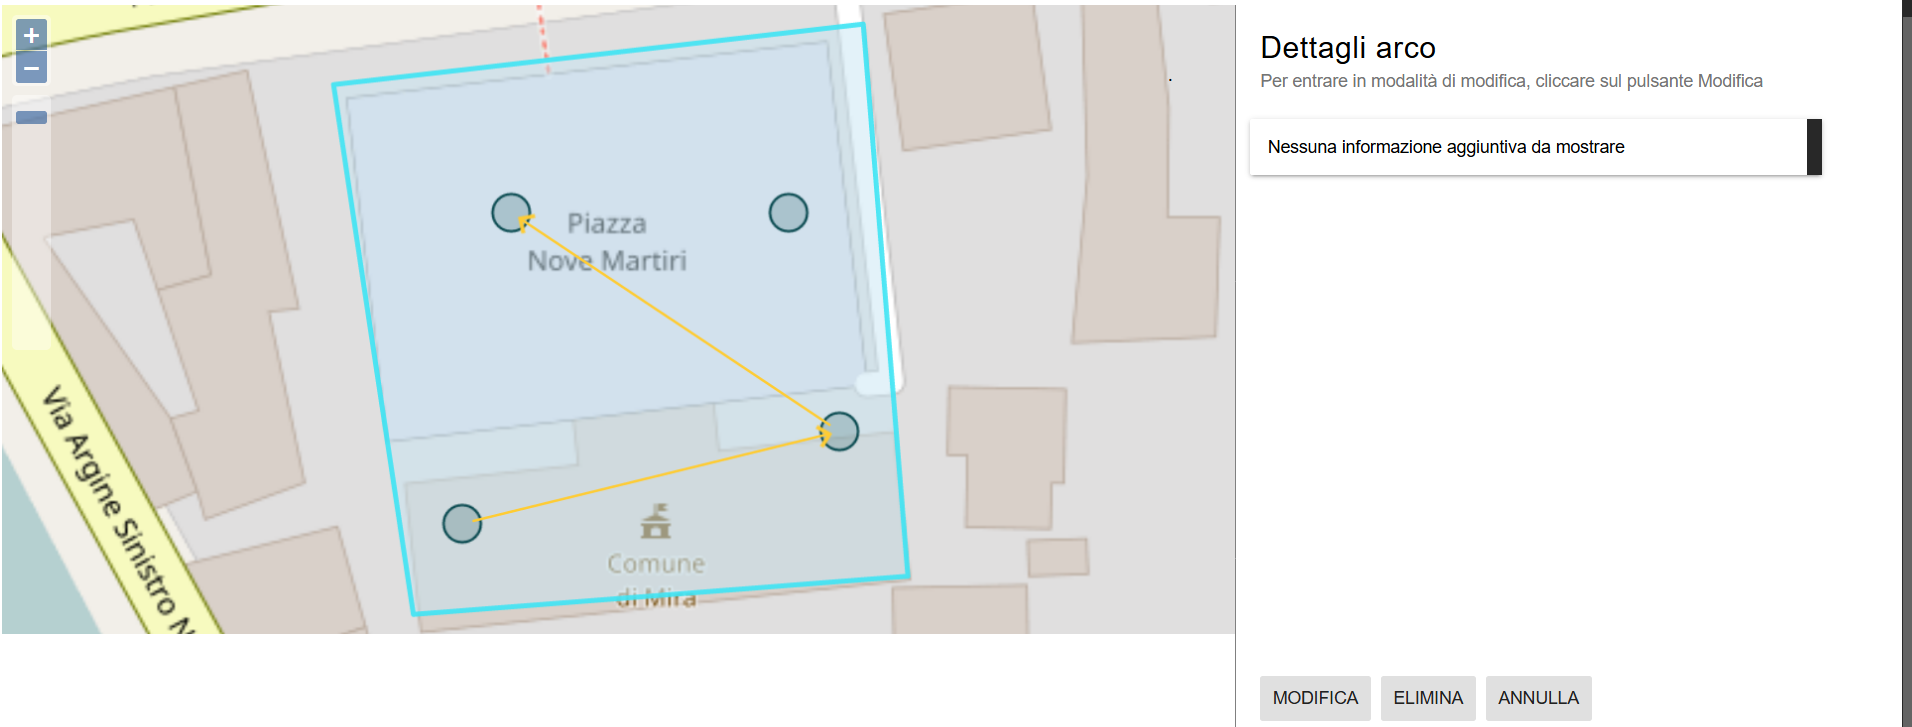
\includegraphics[width=\textwidth]{img/visualizzazione_arco.png}
\caption{Visualizzazione dettagli di un arco}
\end{figure}

\subsection{Modifica di un arco}
Per modificare un arco si deve:
\begin{itemize}
	\item selezionare l'arco che si intende modificare cliccando direttamente sulla mappa;
	\item cliccare sul pulsante "Modifica" in basso sulla sidebar;
	\item eventualmente selezionare il nodo di inizio e il nodo di fine sulla mappa. Il nuovo arco tracciato andrà in automatico a sovrascrivere quello precedentemente presente;
	\item cliccare sul pulsante "Salva", che verrà abilitato solo nel momento in cui tutte le operazioni sopra descritte sono state eseguite in maniera corretta.
\end{itemize}

\begin{figure}[H]
\centering
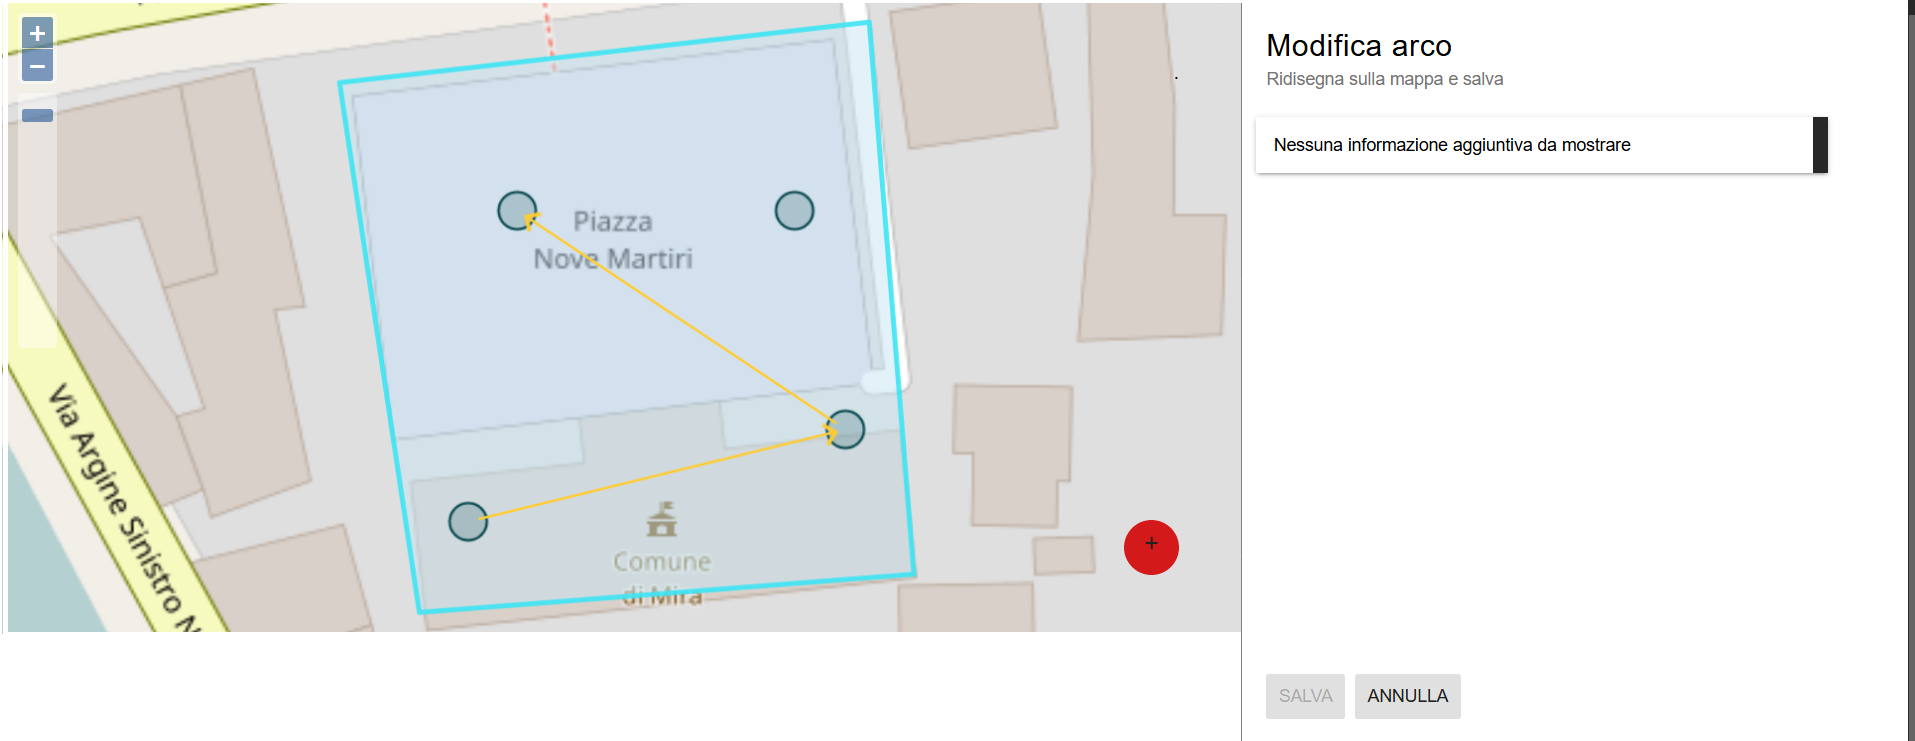
\includegraphics[width=\textwidth]{img/modifica_arco.png}
\caption{Modifica di un arco}
\end{figure}

\subsection{Eliminazione di un arco}
Per eliminare un arco si deve:
\begin{itemize}
	\item selezionare l'arco che si intende modificare cliccando direttamente sulla mappa;
	\item cliccare sul pulsante "Elimina" in basso sulla sidebar;
	\item cliccare sul pulsante "Elimina" sulla finestra bloccante che compare.
\end{itemize}

\begin{figure}[H]
\centering
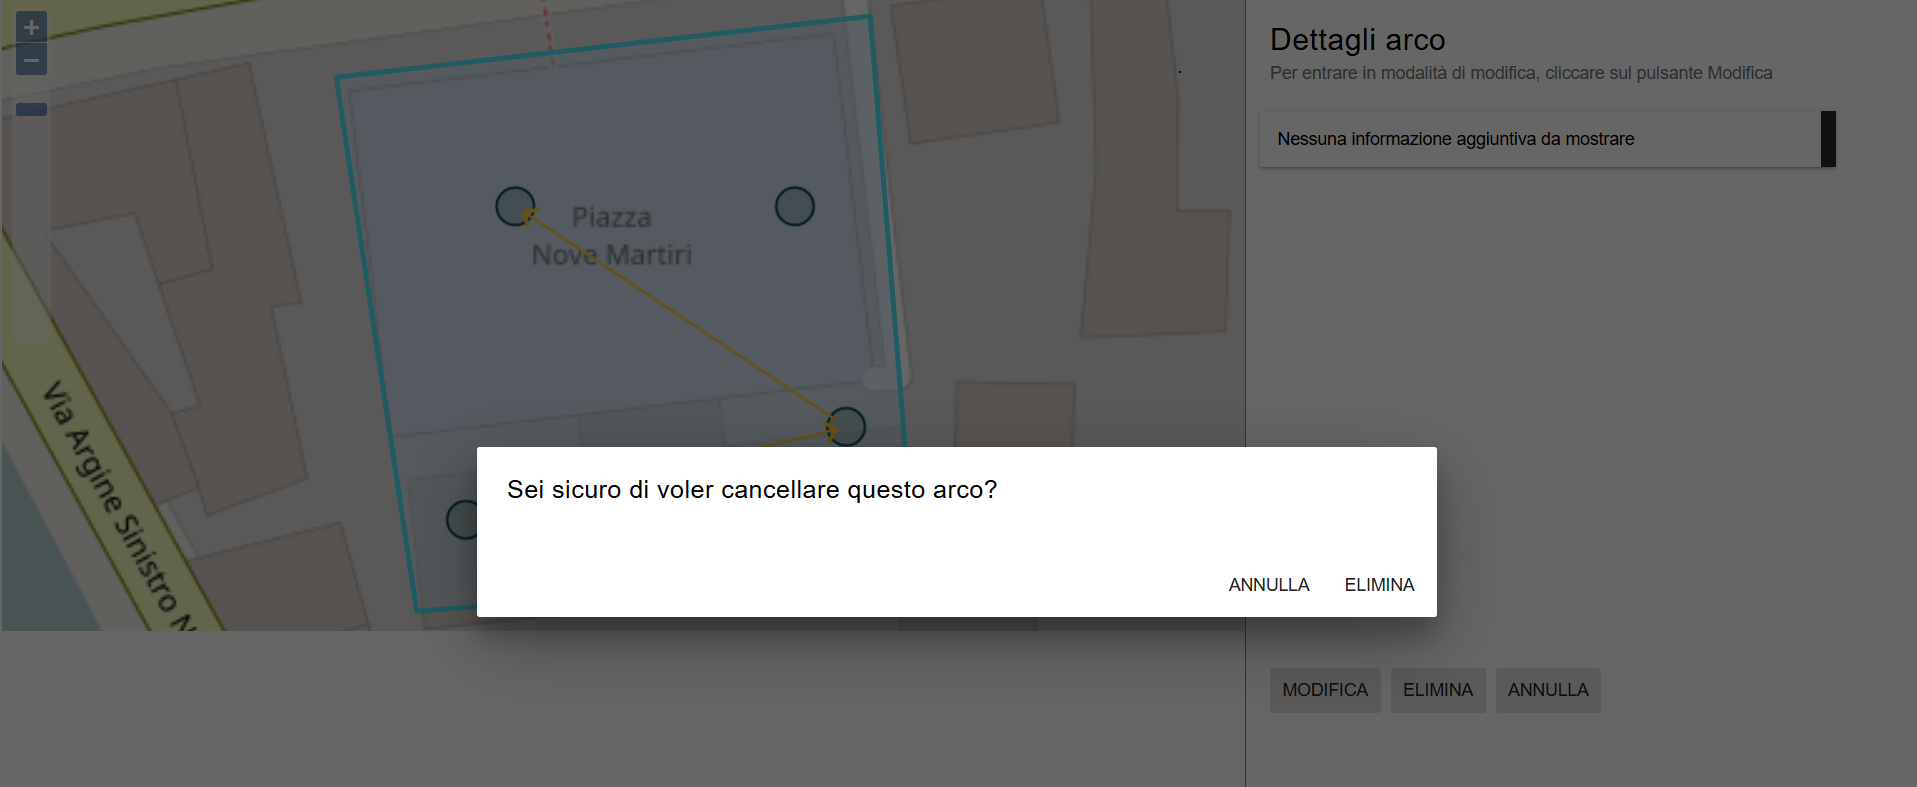
\includegraphics[width=\textwidth]{img/eliminazione_bloccante_arco.png}
\caption{Eliminazione di un arco}
\end{figure}